\chapter{Návrh}

\section{Návrh způsobu specifikace pravidel}

Abychom mohli specifikovat pravidla, musíme nejprve definovat strukturu, nad kterou budou tato pravidla platit. V tomto textu formalizujeme model programu pomocí teorie grafů. Nad grafem je možné dále specifikovat pravidla, která musí vstupní projekt splňovat.

\subsection{Formalizace modelu programu pomocí grafu}
\label{design-graph_formalization}

Analyzovaný softwarový projekt abstrahujeme jako orientovaný multigraf rozšířený o zobrazení množiny uzlů do množiny typů a zobrazení hran do množiny jejich klasifikátorů (označení typu vztahu mezi uzly). Získáme tak následující strukturu:

\begin{displaymath}
G = \langle V, E, \rho, K, C, \mathit{Kind}, \mathit{Class}\rangle
\label{extended_multigraph}
\end{displaymath}
v níž platí:
\begin{itemize}
\item $V$ je množina elementů (v našem případě části kódu)
\item $E$ je množina hran (v našem případě vztahy mezi částmi kódu - např. volání funkce, dědičnost)
\item $V \cap E = \emptyset$
\item $\rho: E \mapsto V \times V$ je zobrazení množiny hran do množiny uspořádaných dvojic vrcholů (incidence)
\item $K$ je libovolná množina označení typů vrcholů\footnote{Pod pojmem typ zde rozumíme jakékoliv označení, které specifikuje o jaký objekt se jedná -- může to být třída, metoda, příkaz, \ldots},
\item $\mathit{Kind}: V \mapsto K$ je zobrazení, které přiřadí každému vrcholu jeho typ,
\item $C$ je množina klasifikátorů hran,
\item $\mathit{Class}: E \mapsto C$ je zobrazení, které přiřadí každé hraně její klasifikátor (zda se jedná o \emph{method call}, \emph{dědičnost}, atd.)
\end{itemize}

Ukázka formalizace zdrojového kódu pomocí grafu je na obrázku \ref{design-graph_example}. V uvedeném příkladě můžeme strukturu $G$ namapovat následujícím způsobem:
\begin{figure}[h!]
  \centering
  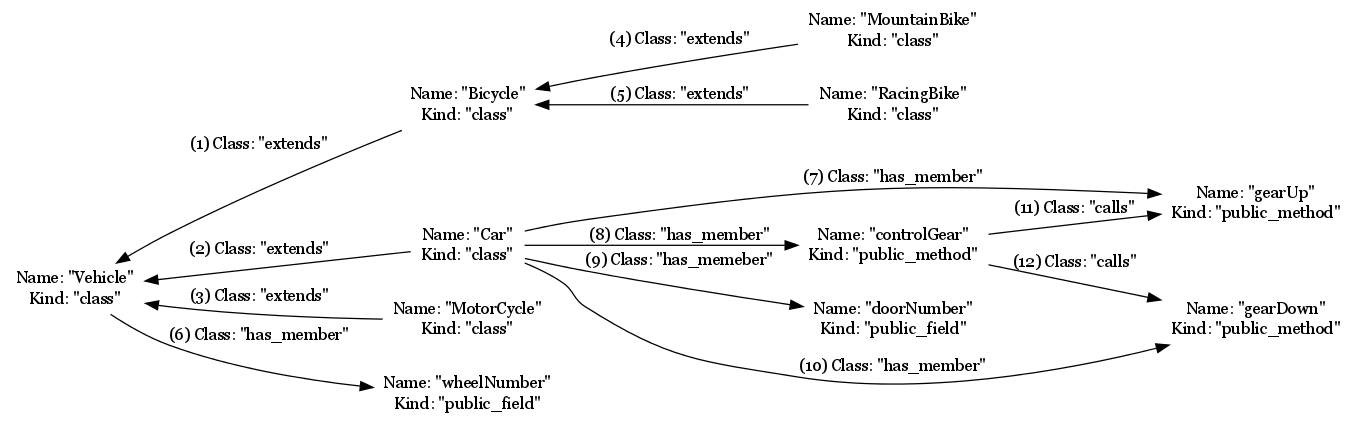
\includegraphics[width=1.0\textwidth]{./graphs/graph_example.png}
  \caption{Příklad formalizace hierarchie tříd jako grafu.\label{design-graph_example}}
\end{figure}
Množinu vrcholů můžeme ztotožnit s množinou názvů elementů (v našem případě třídy, pole, metody).
\begin{align*}
V = &\{ \\
&Vehicle, Car, MotorCycle, Bicycle, MountainBike, RacingBike, \\
&wheelNumber, doorNumber, \\
&controlGear, gearUp, gearDown \\
&\}
\end{align*}
Abychom mohli demonstrovat množinu hran, bylo provedeno očíslování. Hranu zde identifikujeme číslem. V počítačové reprezentaci se může jednat o konkrétní objekt uložený v poli. Množinu hran potom můžeme reprezentovat prostým výčtem čísel:
\begin{displaymath}
E = \{1, 2, 3, 4, 5, 6, 7, 8, 9, 10, 11, 12\}
\end{displaymath}
Zobrazení $\rho$ můžeme formálně zapsat jako následující množinu\footnote{Zobrazení je binární relace. Proto jej můžeme reprezentovat jako množinu uspořádaných dvojic.}:
\begin{align*}
\rho = &\{ \\
&(1, (Bicycle, Vehicle)), \\
&(2, (Car, Vehicle)), \\
&(3, (MotorCycle, Vehicle)), \\
&(4, (MountainBike, Bicycle)), \\
&(5, (RacingBike, Bicycle)), \\
&(6, (Vehicle, wheelNumber)), \\
&(7, (Car, gearUp)), \\
&(8, Car, controlGear)), \\
&(9, (Car, doorNumber)), \\
&(10, (Car, gearDown)), \\
&(11, (controlGear, gearUp)), \\
&(12, (controlGear, gearDown)) \\
&\}
\end{align*}
Zbývají nám množina typů $K$,
\begin{align*}
K = \{ class, public\_field, public\_method \}
\end{align*}
množina klasifikátorů hran $C$,
\begin{align*}
C = \{ \langle\langle{}extends\rangle\rangle, \langle\langle{}has\_member\rangle\rangle, \langle\langle{}calls\rangle\rangle \}
\end{align*}
přiřazení typů uzlům $Kind$,
\begin{align*}
Kind = &\{ \\
&(Bicycle, class), \\
&(Car, class), \\
&(MotorCycle, class), \\
&(MountainBike, class), \\
&(RacingBike, class), \\
&(Vehicle, class), \\
&(wheelNumber, public\_field), \\
&(doorNumber, public\_field), \\
&(controlGear, public\_method), \\
&(gearUp, public\_method), \\
&(gearDown, public\_method) \\
&\}
\end{align*}
a přiřazení klasifikátorů hranám:
\begin{align*}
Class = &\{ \\
&(1, \langle\langle{}extends\rangle\rangle), \\
&(2, \langle\langle{}extends\rangle\rangle), \\
&(3, \langle\langle{}extends\rangle\rangle), \\
&(4, \langle\langle{}extends\rangle\rangle), \\
&(5, \langle\langle{}extends\rangle\rangle), \\
&(6, \langle\langle{}has\_member\rangle\rangle), \\
&(7, \langle\langle{}has\_member\rangle\rangle), \\
&(8, \langle\langle{}has\_member\rangle\rangle), \\
&(9, \langle\langle{}has\_memeber\rangle\rangle), \\
&(10, \langle\langle{}has\_member\rangle\rangle), \\
&(11, \langle\langle{}calls\rangle\rangle), \\
&(12, \langle\langle{}calls\rangle\rangle), \\
\}
\end{align*}

%% Graf elementů použitých v kódu. Vrcholy $v \in V$ představují různé syntaktické elementy v analyzovaném kódu. Záleží na úrovni prováděné analýzy, jaké zvolíme vrcholy. V případě, že budeme analyzovat \uv{nízkoúrovňové} chování funkce, mohou být vrcholy jednotlivé příkazy a jejich části. Pokud budeme analyzovat míru provázanosti tříd nebo metod, stačí když použijeme jako vrcholy třídy a metody (případně parametry metod.)
%% $G = (V, E)$

\subsection{Formalizace pravidel}

\begin{itemize}
\item definice jazyka pro specifikaci pravidel
\item specifikovat množinu objektů, nad nimiž budou pravidla stavěna -- nad čím budeme operovat (možnosti: gramatika, třídy, FJ, graf, \ldots)
\item lze vyjít z Java Language Specification (množina neterminálních a terminálních symbolů)
\item může být nějaký DSL
\end{itemize}

\subsection{Typy pravidel}
\begin{itemize}
\item pravidla definovaná ve vytvořeném formalismu (DSL rules)
\item uživatelsky programovaná pravidla (custom code java code, asserts)
\end{itemize}

TODO: zapracovat:

Ne všechna pravidla lze popsat exaktně ve smyslu splněno/nesplněno. Mnohdy můžeme kvalitu návrhu posuzovat pouze kvantitativně (dobrý návrh, lepší, moc vazeb, málo vazeb, atd.). Pro některé vlastnosti návrhu (např. low coupling, high cohesion) může být vhodnější poskytnou statistický přístup pro vyhodnocování (např. použití vhodného klasifikátoru).

\section{Návrh architektury systému}
TODO: highlevel design $\rightarrow$ jaké budou moduly a co budou dělat (zatím bez konkrétní použité technologie)

% NOTE: při zpracování většího projektu bude nejspíš nutné zavést nad jmény objektů vhodnou formu indexace pro zrychlení algoritmů (kanonická jména tříd jsou v javě poměrně dost dlouhá)

\begin{itemize}
\item compiler
\item generátor vnitřní struktury (modelu) -- modelem je v našem případě graf
\begin{itemize}
\item \emph{vstup:} množina cest k \verb+*.java+ souborům (kompilačním jednotkám), z nichž se skládá softwarový projekt
\item \emph{výstup:} graf, reprezentující konkrétní analyzovanou doménu vhodný pro další zpracování (graf podle \ref{design-graph_formalization} \nameref{design-graph_formalization})
\end{itemize}
\item možnosti generování grafu závislostí mezi třídami (vnitřní reprezentace):
  \begin{itemize}
  \item on demand -- když bude potřeba, vybuduje se kompletně celý graf a poté se zahodí
  \item on the fly -- při práci uživatele na kódu se bude vždy generovat znovu celý graf
  \item kombinovaný přístup -- graf se ve vhodných okamžicích celý vybuduje a poté budou probíhat jeho následné aktualizace na základě uživatelovy práce nad kódem
  \end{itemize}
\item analyzátor
\item rozhraní - integrace do platformy NetBeans
  \begin{itemize}
  \item rozhraní pro zadávání pravidel
  \item rozhraní pro ověřování platnosti pravidel (validaci)
  \end{itemize}
\end{itemize}

% TODO: navrhnout aplikaci tak, aby mela vice rozhrani (nejen GUI, ale i moznost integrace, moznost textoveho vstupu pravidel)

\section{Návrh rozhraní pro zadávání pravidel}
%% rozhraní pro zadávání pravidel bude dáno jazykem, který se pro definici pravidel bude používat - možná kompilátor DSL jazyka, výrazy, atd.
\begin{itemize}
\item rozhraní pro zadávání pravidel
\item formát zadávání pravidel (serializace formalismu tak, aby jej bylo možné textově nebo jinak zadávat)
\end{itemize}

\section{Návrh rozhraní pro ověřování platnosti pravidel (validaci)}
\begin{itemize}
\item výstupní rozhraní
\item validační události
\end{itemize}

%% TODO:
% typy grafů: class hierarchy graph, call graph
% call graph: wikipedia (<<invokes>> vazby)
%
% http://en.wikipedia.org/wiki/Call_graph
%

%% TODO: dat na spravne misto
\section{Návrh technologií pro implementaci}
\begin{itemize}
\item NetBeans platform
\item Maven project
\item Java 1.6
\item \ldots
% TODO: vytvorit prehled technologii i s jejich popisy
\end{itemize}
